\begin{figure*}
\centering
\includegraphics[width=\textwidth]{res_flux_FHR}
\caption{\label{fig:res-flux-FHR}Relative flux enhancements of $E$ (left column), $L_z$ (middle) and $Q$ (right) for resonance ratios corresponding to the 1:3, 1:2, 2:3 and 3:4 resonances. We show results as computed here with a solid red line, and results from Flanagan, Hughes and Ruangeri (FHR14)~\cite{Flanagan2012a} with a dashed blue line. Each row has a different eccentricity and inclination corresponding to tables I--IV in FHR14. All systems have $a_\ast=0.9$.}
\end{figure*}

The plus-polarisation of the GW at the start and end of the evolution is shown in the top row of \figref{good-waveform}.
\begin{figure*}
\centering
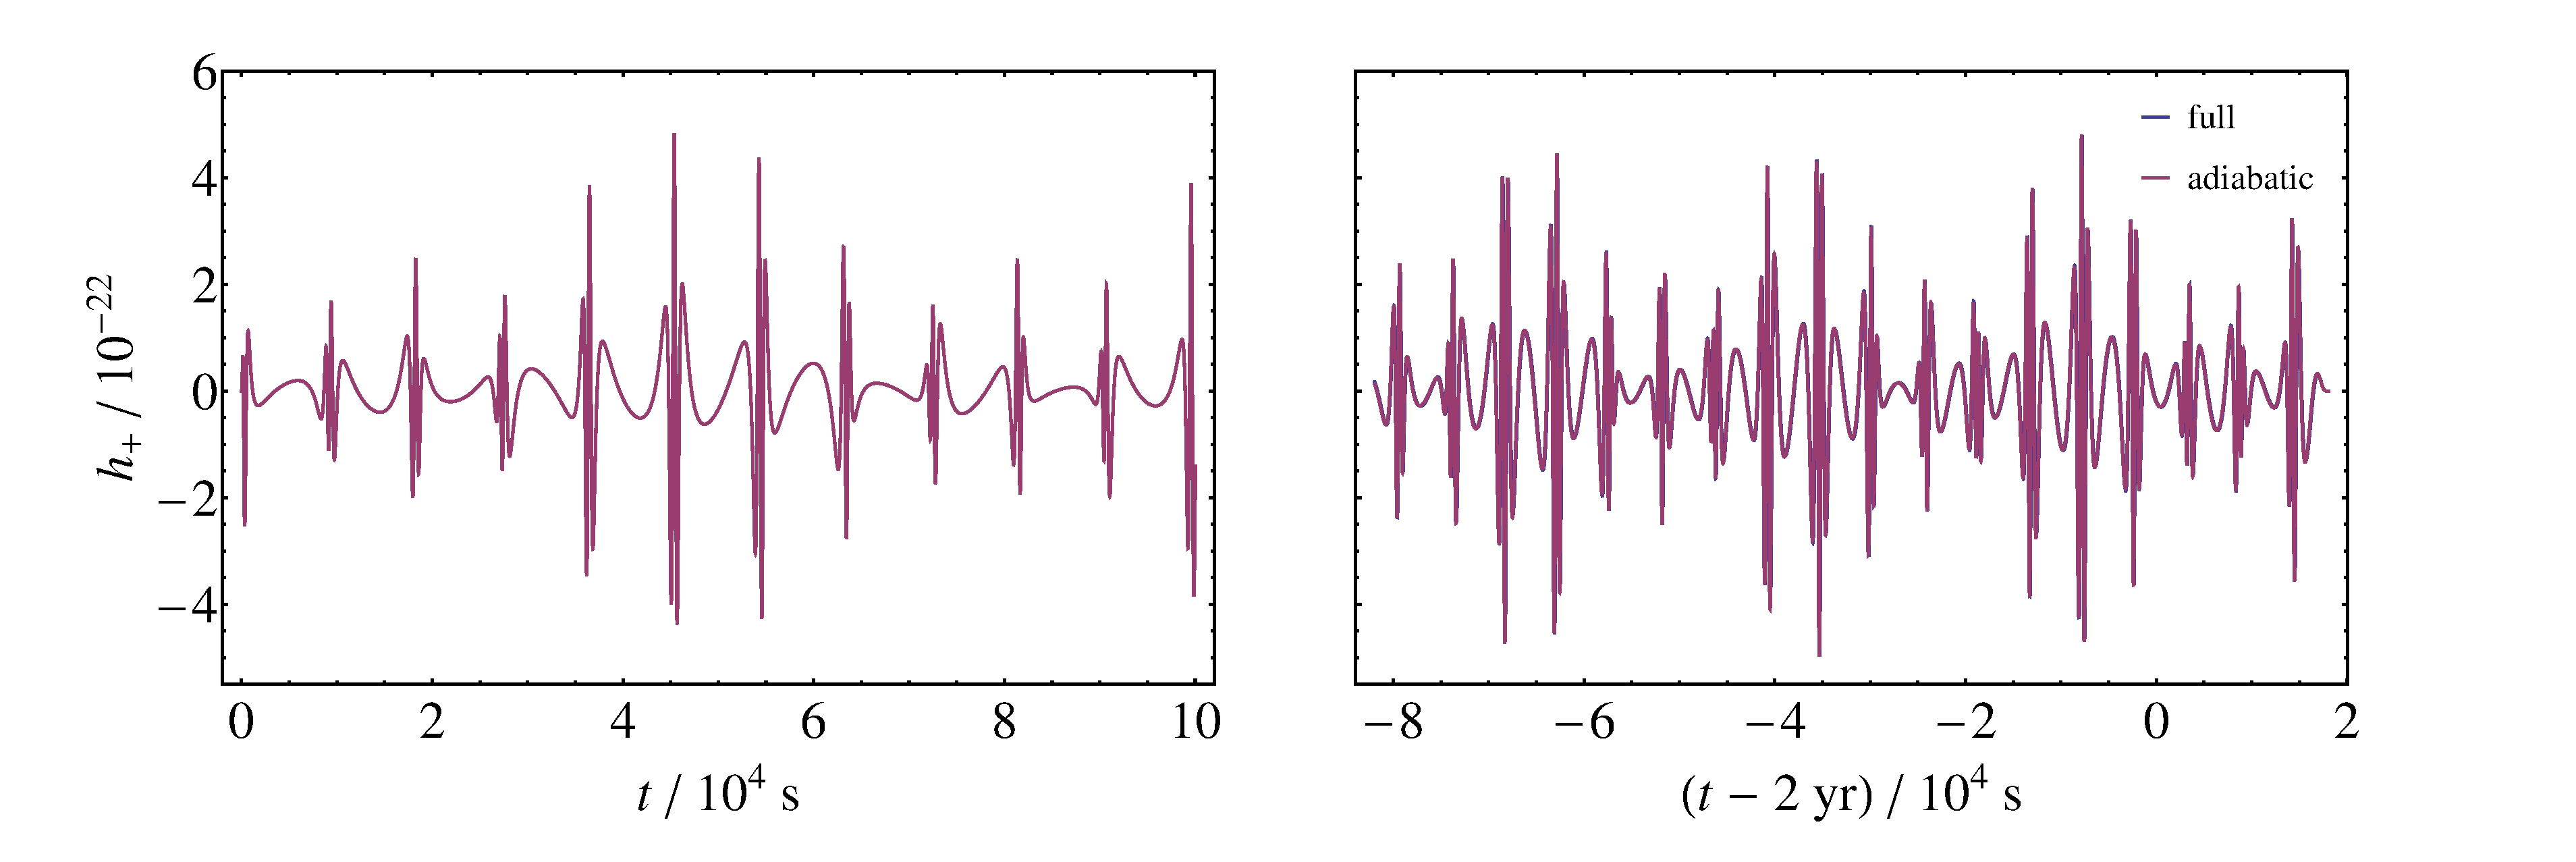
\includegraphics[width=0.92\textwidth]{Fig_good_waveform}
\caption{\label{fig:good-waveform}The plus-polarised waveform for an illustrative EMRI system with initial semi-latus rectum $p_0=7.5$, shown for two short segments at the start and end of a $2$ year evolution. The full and adiabatic models are both shown, but are indistinguishable by eye.}
\end{figure*}

Plotting the plus-polarised GWs at the start and end of the evolution, as before, demonstrates this dephasing, as shown in \figref{dephased-waveform}.
\begin{figure*}
\centering
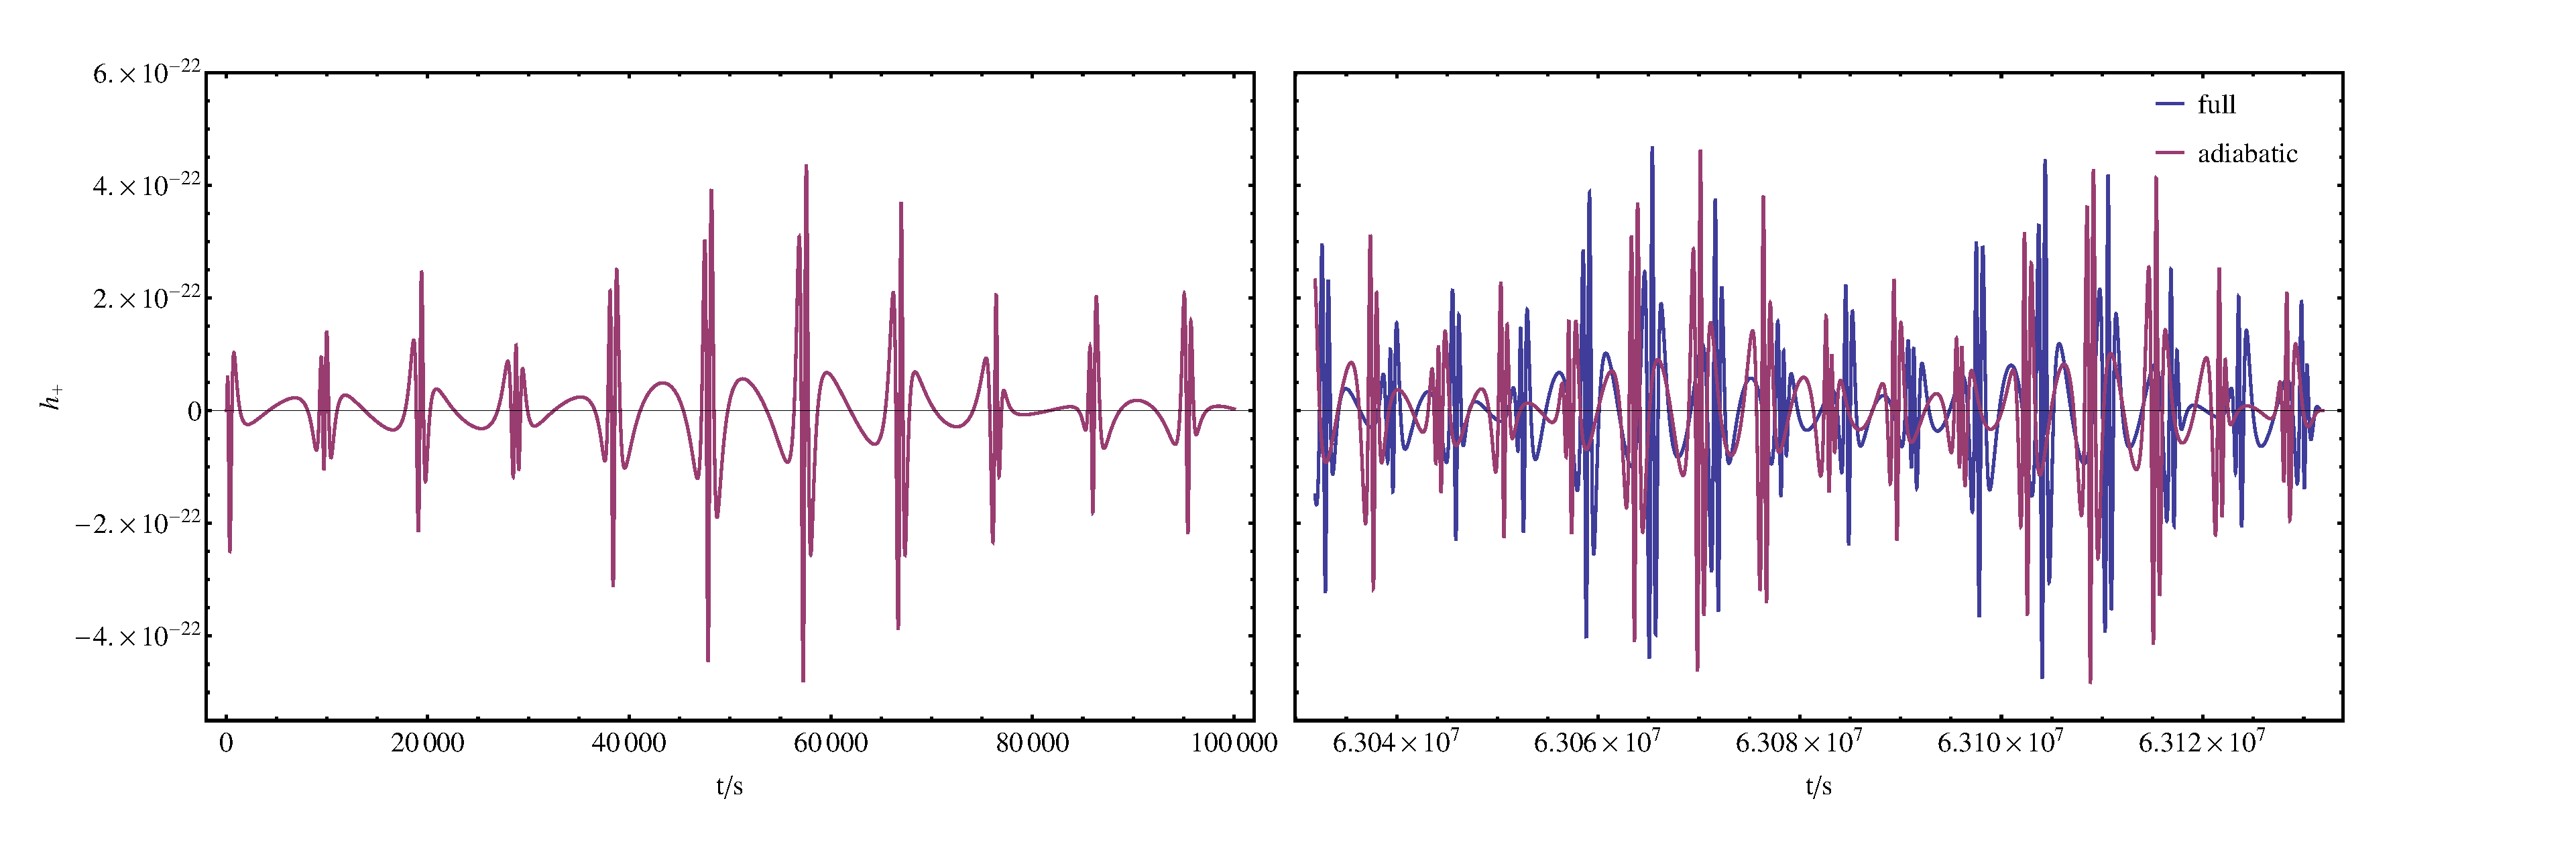
\includegraphics[width=0.92\textwidth]{Fig_dephased_waveform}
\caption{\label{fig:dephased-waveform}The plus-polarised waveform for an illustrative EMRI system with $p=7.85$, shown for two short segments at the start and end of a $2$ year evolution. The full and adiabatic models are both shown; there is a significant dephasing between them by the end of the evolution.}
\end{figure*}

For each system, we compute the overlap between the full evolution and the family of adiabatics given by our set of match times $t\sub{match}$ described in the previous section. The largest overlap in each case, plotted in \figref{overlap-vs-q}, appears to be roughly independent of the value of $q$ and hence with the relative sizes of the orbital parameter jumps.
\begin{figure}
\centering
\includegraphics[width=0.46\textwidth]{overlap_vs_q}
\caption{\label{fig:overlap-vs-q}The overlap between the full and adiabatic evolutions, maximised over the family of generated adiabatics, as a function of the extracted phase parameter $q$. Each dot represents a system with our illustrative parameters and a random choice of the initial radial phase. The red line indicates the expected overlap assuming that the waveforms match exactly post-resonance, but have zero overlap pre-resonance.}
\end{figure}
The best performing adiabatic for the majority of our systems matched at the end of the inspiral. We can therefore estimate the value of the overlap by assuming that the adiabatic waveforms recover the entire SNR in the region post-resonance, but none at all in the region pre-resonance. We expect the overlap to scale with the fraction of time spent post-resonance, the value of which is demonstrated by the red line in \figref{overlap-vs-q}. There is not an exact equivalence because of the frequency-dependent noise of eLISA; cycles near the end of the inspiral accumulate proportionally more SNR at a frequency closer to the minimum of the eLISA noise curve.
Systems with $|q| \approx \pi/2$ (corresponding to small jumps in $E$ and $L_z$) have higher than average overlaps due to additional accumulation in the pre-resonance region. The adiabatic models of these systems dephase more slowly, but still do not produce very high overlaps due to the jump in $Q$. A small fraction of systems have a lower overlap than expected, at around $0.5$. This is due to a sub-optimal choice of the matching times; making small adjustments to $t\sub{match}$ can lead to higher overlaps, but the exact adjustments required are difficult to predict in advance.
